% ============================================================
%  template-8min.tex —— 8 分钟进站考核精简版（先写 Part 1）
%  内容定稿见 outline-8min.md；原 28 帧完整版见 template.tex（素材库）
%  编译方式：XeLaTeX（支持中文），编译两次生成目录
% ============================================================
\documentclass[notheorems]{beamer}

\input{pptheader.tex}
\input{mycommand.tex}

% ============================================================
%  无框风格辅助命令（本精简版专用）
% ============================================================
% 小节标题：粗体彩色字 + 细分隔线
\newcommand{\blocktitle}[1]{%
	{\fontsize{10}{12}\selectfont\bfseries\sffamily\color{structure.fg}#1}\\[3pt]%
	{\color{structure.fg!35}\rule{\linewidth}{0.8pt}}\\[6pt]}
% 引导/总述：左侧色条 + 文字（替代 panelbg 总述条）
\newcommand{\accentintro}[1]{%
	\noindent{\color{structure.fg}\rule[-2pt]{3pt}{12pt}}\hspace{7pt}%
	\begin{minipage}[t]{\dimexpr\linewidth-13pt\relax}%
		\fontsize{8}{11.5}\selectfont\sffamily #1\end{minipage}\par}
% 结论 takeaway：居中粗体彩色一句（替代深色结论条）
\newcommand{\takeaway}[1]{%
	\begin{center}{\fontsize{9}{13.5}\selectfont\sffamily\bfseries\color{structure.fg}#1}\end{center}}
% 图注小标题：粗体彩色（替代图卡片色头）
\newcommand{\imglabel}[1]{%
	{\fontsize{8}{10}\selectfont\sffamily\bfseries\color{structure.fg}#1}\par\vspace{2pt}}

\begin{document}

	% ============================================================
	%  元信息
	% ============================================================
	\title[科研汇报]{结构拓扑优化的高精度数值方法与高性能求解}
	\subtitle{博士后进站考核 · 科研工作汇报与研究计划}

	\author[何亮]{报告人：何亮 \\
		\vspace{5pt}
		博士导师：{\CJKfontspec{SimSun}魏华祎} 教授 \\
		\vspace{2pt}
		合作导师：{\CJKfontspec{SimSun}郭旭} 院士}

	\institute[湘大\,·\,大工]{
		\vspace{5pt}
		湘潭大学 数学与计算科学学院\,（博士）\\
		大连理工大学 力学与航空航天学院\,（博士后）
	}
	\date{\today}

	% ---- 封面页 ----
	\frame[plain]{\titlepage}

	% ============================================================
	%  帧 1 · 个人简介（开场帧）
	% ============================================================
	\begin{frame}[plain]

		\begin{tikzpicture}[remember picture, overlay]
			\fill[structure.fg]
			(current page.north west)
			rectangle ([yshift=-0.077\paperheight] current page.north east);
			\node[white, anchor=west, font=\small\bfseries\sffamily]
			at ([xshift=0.025\paperwidth, yshift=-0.038\paperheight]
			current page.north west)
			{个人简介};
			\fill[panelbg]
			([yshift=-0.077\paperheight] current page.north west)
			rectangle ([xshift=0.38\paperwidth] current page.south west);
		\end{tikzpicture}

		\vspace{0.077\paperheight}

		\begin{columns}[T, totalwidth=\linewidth]

			% ══════════════════════════════════════════
			% 左栏：照片 + 姓名 + 研究方向 + 教育/工作经历
			% ══════════════════════════════════════════
			\begin{column}{0.36\linewidth}
				\vspace{0.5em}
				\begin{center}
					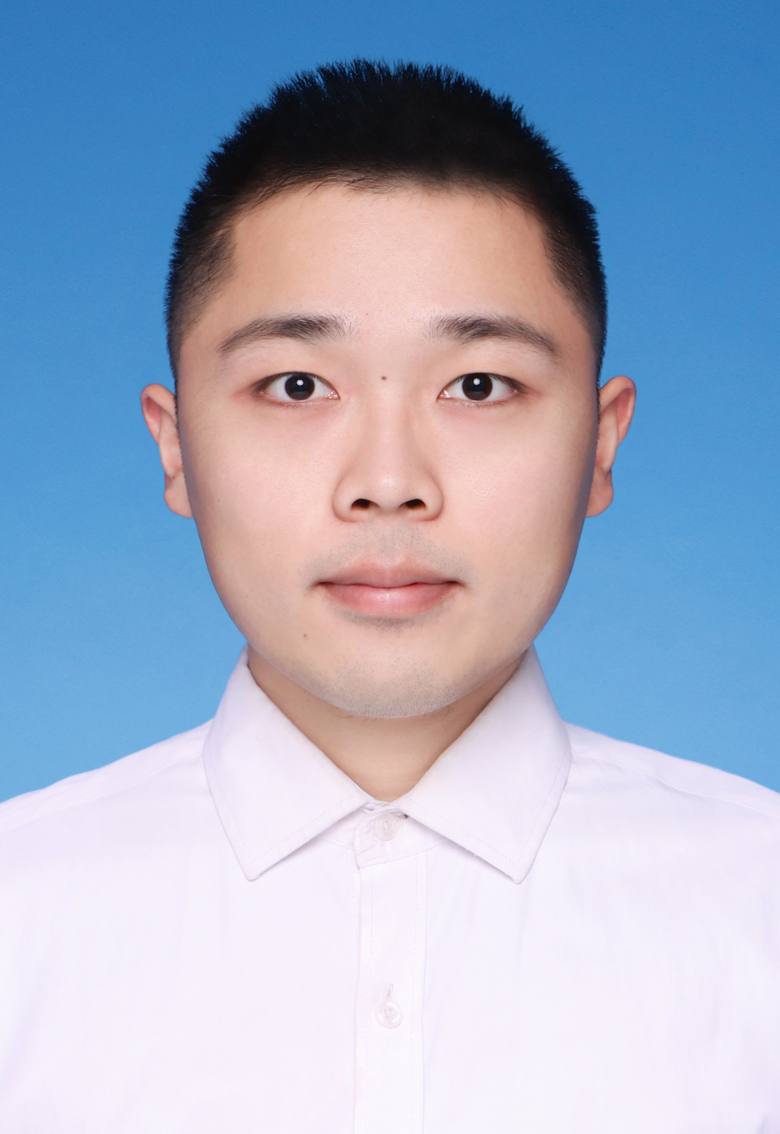
\includegraphics[width=0.50\linewidth,
					height=0.22\paperheight,
					keepaspectratio]{photo.jpg}

					\vspace{0.3em}
					{\fontsize{14}{18}\selectfont\bfseries\sffamily 何\quad 亮}

					\vspace{0.6em}
					{\fontsize{9.5}{12}\selectfont\bfseries\sffamily\color{structure.fg}研究方向}\\[2pt]
					{\color{structure.fg!35}\rule{0.78\linewidth}{0.7pt}}

					\vspace{5pt}
					{\fontsize{8.5}{15}\selectfont\sffamily\color{structure.fg}
						偏微分方程数值方法\\
						连续体结构拓扑优化\\
						科学计算软件设计与实现}
				\end{center}
			\end{column}

			% ══════════════════════════════════════════
			% 右栏：研究主线 + 研究目标
			% ══════════════════════════════════════════
			\begin{column}{0.62\linewidth}
				\vspace{0.5em}

				% ── 博士阶段·研究主线（无框）──────────────
				\blocktitle{博士阶段\,·\,研究主线}

				{\fontsize{7.5}{10}\selectfont\sffamily
					围绕基于高阶有限元的变密度拓扑优化，重点关注四个方面：}

				\vspace{6pt}
				\begin{tabular}{@{}l@{\hspace{3pt}}p{3.0cm}@{\hspace{10pt}}l@{\hspace{3pt}}p{3.0cm}@{}}
					\circnum{01} & {\fontsize{7.5}{9.5}\selectfont\sffamily 高阶有限元拓扑优化方法} &
					\circnum{03} & {\fontsize{7.5}{9.5}\selectfont\sffamily 胡张混合有限元拓扑优化方法} \\[7pt]
					\circnum{02} & {\fontsize{7.5}{9.5}\selectfont\sffamily 多分辨率拓扑优化框架} &
					\circnum{04} & {\fontsize{7.5}{9.5}\selectfont\sffamily SOPTX 软件平台设计与实现} \\
				\end{tabular}

				\vspace{12pt}
				% ── 博士后·研究方向（无框）────────────────
				\blocktitle{博士后\,·\,研究方向}

				\begin{tabular}{@{}l@{\hspace{4pt}}p{\dimexpr\linewidth-1.1cm\relax}@{}}
					\circnum{01} & {\fontsize{7.5}{10.5}\selectfont\sffamily PIML 增强多尺度结构分析与 Matrix-Free 高性能求解} \\[7pt]
					\circnum{02} & {\fontsize{7.5}{10.5}\selectfont\sffamily MMC/MMV 显式拓扑优化的高精度数值离散与高效结构分析} \\
				\end{tabular}

			\end{column}
		\end{columns}
	\end{frame}


	% ============================================================
	\section{一、博士期间研究工作}
	% ============================================================

	% ============================================================
	%  帧 2 · 方法一 · 任意次拉格朗日高阶有限元
	%  （合并 任意次拉格朗日FEM 总述 + 阶次对比结果）
	% ============================================================
	\begin{frame}
		\frametitle{方法一 · 任意次拉格朗日高阶有限元}

		% ── 顶部引导（无框）──
		\accentintro{将状态方程从低阶位移元推广到\textbf{任意次拉格朗日有限元 $V_h^k$}，提升位移场及派生应力场逼近精度；以二维对称 MBB 梁为基准（统一四边形单元、体积约束、无过滤）考察离散阶次的影响。}

		\vspace{0.7em}

		% ── 三栏：阶次对比 k=1/2/4（无框）──
		\begin{columns}[T, totalwidth=\linewidth]

			\begin{column}{0.325\linewidth}\centering
				\imglabel{\circnum{01}\enspace 线性元 $k = 1$}
				
\includegraphics[width=\linewidth, height=0.265\paperheight, keepaspectratio]{topo_k1}\\[3pt]
				{\fontsize{7.5}{11}\selectfont\sffamily $n = 53,\ c \approx 203.07$\\ 棋盘格现象明显，边界锯齿化突出}
			\end{column}

			\begin{column}{0.325\linewidth}\centering
				\imglabel{\circnum{02}\enspace 二阶元 $k = 2$}
				
\includegraphics[width=\linewidth, height=0.265\paperheight, keepaspectratio]{topo_k2}\\[3pt]
				{\fontsize{7.5}{11}\selectfont\sffamily $n = 36,\ c \approx 213.18$\\ 构型质量明显改善，局部伪结构减少}
			\end{column}

			\begin{column}{0.325\linewidth}\centering
				\imglabel{\circnum{03}\enspace 四阶元 $k = 4$}
				
\includegraphics[width=\linewidth, height=0.265\paperheight, keepaspectratio]{topo_k4}\\[3pt]
				{\fontsize{7.5}{11}\selectfont\sffamily $n = 41,\ c \approx 218.66$\\ 相较 $k=2$ 改善有限，拓扑细节未同步提升}
			\end{column}

		\end{columns}

		\vspace{0.9em}

		% ── 结论（无框）──
		\takeaway{提高分析阶次具有一定改善作用，但其收益受单分辨率设计空间限制 $\Rightarrow$ 引入多分辨率解耦}

	\end{frame}

	% ============================================================
	%  帧 3 · 方法二 · 高阶多分辨率拓扑优化框架
	%  （合并 单分辨率精度错配[动机] + 多分辨率框架 + 表达优势[数据]）
	% ============================================================
	\begin{frame}
		\frametitle{方法二 · 高阶多分辨率拓扑优化框架}

		% ── 引导（无框）──
		\accentintro{单分辨率框架下设计与分析模型刚性绑定，分析精度与设计分辨率单侧提升难以兼顾；为此引入\textbf{“位移网格 — 密度积分网格 — 设计变量网格”}三层离散体系。}

		\vspace{0.4em}

		% ── 中部：三层网格示意图 ──
		\begin{center}
			
\includegraphics[width=0.88\linewidth, height=0.26\paperheight,
			keepaspectratio]{multires_framework}
		\end{center}

		\vspace{-1.0em}

		% ── 三栏说明（无框：彩色标签 + 文字）──
		\begin{columns}[T, totalwidth=\linewidth]

			\begin{column}{0.32\linewidth}\centering
				{\fontsize{8.5}{11}\selectfont\sffamily\bfseries\color{structure.fg}$\mathcal{T}_h$\enspace 高阶位移网格}\par\vspace{3pt}
				{\fontsize{7.5}{11}\selectfont\sffamily 采用\textbf{较粗高阶位移单元}，控制分析自由度规模}
			\end{column}

			\begin{column}{0.32\linewidth}\centering
				{\fontsize{8.5}{11}\selectfont\sffamily\bfseries\color{structure.fg}$\mathcal{T}_\rho$\enspace 密度积分网格}\par\vspace{3pt}
				{\fontsize{7.5}{11}\selectfont\sffamily 进行\textbf{子单元密度积分}，保证刚度组装一致性}
			\end{column}

			\begin{column}{0.32\linewidth}\centering
				{\fontsize{8.5}{11}\selectfont\sffamily\bfseries\color{structure.fg}$\mathcal{T}_d$\enspace 设计变量网格}\par\vspace{3pt}
				{\fontsize{7.5}{11}\selectfont\sffamily 承载\textbf{高分辨率设计变量}，提升拓扑表达能力}
			\end{column}

		\end{columns}

		\vspace{0.9em}

		% ── 结论（无框，含表达优势数据）──
		\takeaway{三层网格解耦在控制计算规模的同时兼顾高精度分析与高分辨率拓扑表达（MBB：设计自由度 $600\!\to\!9600$，构型更清晰、细节更丰富）}

	\end{frame}

	% ============================================================
	%  帧 4 · 方法三 · 任意次胡张混合有限元
	%  （合并 胡张混合方法[总述] + 近不可压抗闭锁结果）
	% ============================================================
	\begin{frame}
		\frametitle{方法三 · 任意次胡张混合有限元}

		% ── 顶部引导（无框）──
		\accentintro{以应力 $\boldsymbol{\sigma}$ 为独立未知量、构造 $H(\mathrm{div})$ 协调对称张量空间的\textbf{任意次胡张混合有限元}（北大胡俊教授方法），嵌入变密度拓扑优化闭环直接获得高精度应力场；下以二维轴承装置对比两类方法。}

		\vspace{0.5em}

		% ── 列标题行 ──
		\begin{columns}[T, totalwidth=\linewidth]
			\begin{column}{0.10\linewidth}\end{column}
			\begin{column}{0.42\linewidth}\centering
				{\fontsize{8.5}{10}\selectfont\sffamily\bfseries\color{structure.fg}
					可压缩材料 \enspace $\nu_0 = 0.3$\par}
			\end{column}
			\begin{column}{0.42\linewidth}\centering
				{\fontsize{8.5}{10}\selectfont\sffamily\bfseries\color{structure.fg}
					近不可压缩材料 \enspace $\nu_0 = 0.4999$\par}
			\end{column}
		\end{columns}

		\vspace{0.2em}

		% ── 第一行：标准位移法 ──
		\begin{columns}[c, totalwidth=\linewidth]
			\begin{column}{0.10\linewidth}\centering
				{\fontsize{8.5}{10}\selectfont\sffamily\bfseries\color{structure.fg}
					标准\\[3pt]位移法\\{\fontsize{6}{8}\selectfont ($k=2$)}}
			\end{column}
			\begin{column}{0.42\linewidth}\centering
				
\includegraphics[width=0.95\linewidth, height=0.178\paperheight, keepaspectratio]{bearing_disp_nu03}\\[2pt]
				{\fontsize{7}{9}\selectfont $c \approx 123.37$ (结构清晰，正常收敛)}
			\end{column}
			\begin{column}{0.42\linewidth}\centering
				
\includegraphics[width=0.95\linewidth, height=0.178\paperheight, keepaspectratio]{bearing_disp_nu4999}\\[2pt]
				{\fontsize{7}{9}\selectfont $c \approx 55.78$ (刚度高估，构型异常)}
			\end{column}
		\end{columns}

		\vspace{0.4em}

		% ── 第二行：胡张混合法 ──
		\begin{columns}[c, totalwidth=\linewidth]
			\begin{column}{0.10\linewidth}\centering
				{\fontsize{8.5}{10}\selectfont\sffamily\bfseries\color{structure.fg}
					胡张\\[3pt]混合法\\{\fontsize{6}{8}\selectfont ($k=2$)}}
			\end{column}
			\begin{column}{0.42\linewidth}\centering
				
\includegraphics[width=0.95\linewidth, height=0.178\paperheight, keepaspectratio]{bearing_mixed_nu03}\\[2pt]
				{\fontsize{7}{9}\selectfont $c \approx 128.45$ (结构清晰，正常收敛)}
			\end{column}
			\begin{column}{0.42\linewidth}\centering
				
\includegraphics[width=0.95\linewidth, height=0.178\paperheight, keepaspectratio]{bearing_mixed_nu4999}\\[2pt]
				{\fontsize{7}{9}\selectfont $c \approx 102.79$ (抗体积闭锁，构型稳定)}
			\end{column}
		\end{columns}

		\vspace{0.6em}

		% ── 结论（无框）──
		\takeaway{胡张混合有限元有效缓解近不可压体积闭锁，并基于协调应力空间支撑局部应力约束的可靠评估。}

	\end{frame}

	% ============================================================
	%  帧 5a · SOPTX 软件平台（架构 + 关键技术 + GPU 加速）
	% ============================================================
	\begin{frame}
		\frametitle{SOPTX 软件平台 · 架构与高性能}

		\vspace{0.6em}

		\begin{columns}[t, totalwidth=\linewidth]

			% ── 左列：总体架构（无框：标题 + 细线 + 缩进正文）──
			\begin{column}{0.47\linewidth}
				{\fontsize{10}{12}\selectfont\bfseries\sffamily\color{structure.fg}总体架构}\\[3pt]
				{\color{structure.fg!35}\rule{\linewidth}{0.8pt}}\\[7pt]
				{\fontsize{8.5}{13.5}\selectfont\sffamily
					\circnum{1}~\textbf{用户交互层}：Python API、算例配置、后处理与可视化。
					\par\vspace{8pt}
					\circnum{2}~\textbf{核心算法层}：插值—分析—正则化—优化闭环编排主流程。
					\par\vspace{8pt}
					\circnum{3}~\textbf{基础后端层}：依托 FEALPy 组装、求解与多后端张量计算。}
			\end{column}

			\hfill

			% ── 右列：关键技术（无框）──
			\begin{column}{0.47\linewidth}
				{\fontsize{10}{12}\selectfont\bfseries\sffamily\color{structure.fg}关键技术}\\[3pt]
				{\color{structure.fg!35}\rule{\linewidth}{0.8pt}}\\[7pt]
				{\fontsize{8.5}{13.5}\selectfont\sffamily
					\circnum{1}~\textbf{高效矩阵组装}：解析预计算 + 张量收缩 + 算子缓存。
					\par\vspace{8pt}
					\circnum{2}~\textbf{自动微分灵敏度}：PyTorch / JAX 自动求复杂目标/约束梯度（与手动一致）。
					\par\vspace{8pt}
					\circnum{3}~\textbf{多后端与异构}：NumPy / PyTorch / JAX 切换，CPU / GPU 可移植。}
			\end{column}

		\end{columns}

		\vspace{1.1em}

		% ── GPU 加速亮点（无框：左侧色条 + 文字）──
		{\fontsize{8.5}{13}\selectfont\sffamily
			{\color{structure.fg}\rule[-1pt]{3pt}{12pt}}\hspace{8pt}%
			\textbf{GPU 异构加速}（三维悬臂梁）：总耗时 $2789.9\,\mathrm{s}\!\to\!636.7\,\mathrm{s}$，
			端到端 \textbf{4.38$\times$}、稳态 \textbf{4.36$\times$}；多后端构型与收敛一致。\par}

		\vspace{1.2em}

		% ── 结论（无框：居中粗体彩色一句）──
		\begin{center}
			{\fontsize{9.5}{14}\selectfont\sffamily\bfseries\color{structure.fg}
				以“分析—优化解耦”为核心，集成 AD、多后端与 GPU 异构，提供高效可扩展的拓扑优化软件支撑。}
		\end{center}

	\end{frame}

	% ============================================================
	%  帧 5b · 博士成果概览（论文 / 软著 / 项目）
	% ============================================================
	\begin{frame}
		\frametitle{博士成果概览}

		% ── 顶部引导（无框）──
		\accentintro{围绕高阶有限元变密度拓扑优化，形成论文、软件著作权与工程项目的完整成果链。}

		\vspace{0.9em}

		\begin{columns}[T, totalwidth=\linewidth]

			% ── 论文（无框）──
			\begin{column}{0.32\linewidth}
				\blocktitle{\circnum{01}\enspace 论文成果}
				{\fontsize{6.6}{9.5}\selectfont\sffamily
					\textbf{一作}：SOPTX: A Modular \& Extensible Framework for Topology Optimization…，\textit{CiCP} 40(2): 525–572.
					\par\vspace{6pt}
					\textbf{合作}：Adaptive FEM for phase field fracture…，\textit{JCAM} 2026, 472: 116732.
					\par\vspace{3pt}
					\hphantom{\textbf{合作}：}FEALPy: Cross-platform Numerical Simulation Engine，\textit{CiCP}（已录用）.}
			\end{column}

			% ── 软件著作权（无框）──
			\begin{column}{0.32\linewidth}
				\blocktitle{\circnum{02}\enspace 软件著作权}
				{\fontsize{6.6}{9.5}\selectfont\sffamily
					\textbf{结构拓扑优化仿真计算软件}\par\vspace{1pt}
					登记号 2025SR0887352；\textbf{第一完成人}.
					\par\vspace{6pt}
					\textbf{建筑结构力学仿真计算软件}\par\vspace{1pt}
					登记号 2024SR0961048；第三完成人.}
			\end{column}

			% ── 工程项目（无框）──
			\begin{column}{0.32\linewidth}
				\blocktitle{\circnum{03}\enspace 工程项目}
				{\fontsize{6.6}{9.5}\selectfont\sffamily
					\textbf{中建五局合作项目}\par\vspace{1pt}
					建筑结构力学 C++ 计算内核，集成中建智拓平台；主要参与人.
					\par\vspace{6pt}
					\textbf{FEALPy 开源引擎}\par\vspace{1pt}
					计算固体力学库底层架构与多本构求解器；主要参与人.}
			\end{column}

		\end{columns}

		\vspace{1.1em}

		% ── 结论（无框）──
		\takeaway{贯通\textbf{“数学模型 — 数值方法 — 软件实现 — 科研实践”}研究链条，为博士后科研计划奠定基础。}

	\end{frame}


	% ============================================================
	%  结束页（临时；Part 2 写完后接到其后）
	% ============================================================
	\begin{frame}[plain]
		\vspace{1.2cm}
		\begin{center}
			{\fontsize{20}{26}\selectfont\bfseries\sffamily\color{structure.fg} Part 1 完 · 待接 Part 2 博士后科研计划}

			\vspace{0.8cm}
			{\color{structure.fg!35}\rule{0.5\linewidth}{0.8pt}}

			\vspace{0.6cm}
			{\fontsize{13}{18}\selectfont\bfseries\sffamily\color{structure.fg} 敬请各位专家老师批评指正！}
		\end{center}
	\end{frame}

\end{document}
